\documentclass[12pt]{article}

% This is the preamble, load any packages you're going to use here
\usepackage{physics} % provides lots of nice features and commands often used in physics, it also loads some other packages (like AMSmath)
\usepackage{siunitx} % typesets numbers with units very nicely
\usepackage{enumerate} % allows us to customize our lists
\usepackage{booktabs}
\usepackage{graphicx}
\usepackage{natbib}
\bibpunct{[}{]}{,}{n}{}{;}




\begin{document}

\title{The Electron Charge to Mass Ratio}
\author{James Amarel}
\date{\today}

\maketitle

\section{Goal}
The goal of this experiment is to test the theory that electrons are negatively charged massive particles by comparing their motion with the predictions of the Lorentz force law. We use a known accelerating voltage to propel electrons into a region of known magnetic field where a phosphorescent mica screen is used to visualize the beam's deflection.

\section{Introduction/Background}
	The properties of cathode rays were a great mystery to scientists of the late 1800s. At the time many physicists resorted to the aether as a scapegoat explanation \cite{Thomson2010CathodeRays}. An under supported theory was that cathode rays were the paths of particles of matter with negative electricity. Supporting evidence for the particle theory emerged when Jean Perrin showed that a cathode ray bulb emitted negative charge \cite{Thomson2010CathodeRays}. Perrin accomplished this by measuring the difference in current through a loop and the absence of current when the ray was deflected. Unbeknownst to Perrin, this wasn't entirely proof that the charged particles were themselves the cathode rays. It was well known that cathode rays did not deflect when in a small electric field and without a way to visualize the beam there was no proof the beam itself was deflected. JJ Thomson corrected for this by tracing the phosphorescence of the ray path as seen through a glass tube. At this point, Aether theory seemed incredibly unlikely and Thomson found no alternative to the conclusion that cathode rays must be "charges of negative electricity carried by particles of matter" \cite{Thomson2010CathodeRays}.
    
We aim to recreate Thomson's famous measurement of the electron's charge to mass ratio by recording the deflection of an electron moving perpendicular to a uniform magnetic field \cite{Griffiths2013IntroductionElectrodynamics}. According to the Lorentz force law, the centripetal force is determined by the product $qvB$ which produces a circular trajectory with constant momentum as given by:


\begin{equation}\label{Cyclotron}
    mv = qBr
\end{equation}

An accelerating potential imparts kinetic energy upon the electrons and aims them to be deflected by the magnetic field. With the assumption that the electrons originate at rest, we can use conservation of energy and equation \ref{Cyclotron} to find a new expression involving the charge to mass ratio:
\begin{equation}\label{Energy}
    r^2 = \frac{2mV_a}{qB^2}
\end{equation}
Evidently, we can manipulate the radius of curvature for the electron path by choice of laboratory controlled values for the accelerating voltage and the magnetic field.  



\section{Procedures and Data}

\begin{figure}[t]
  \centering
  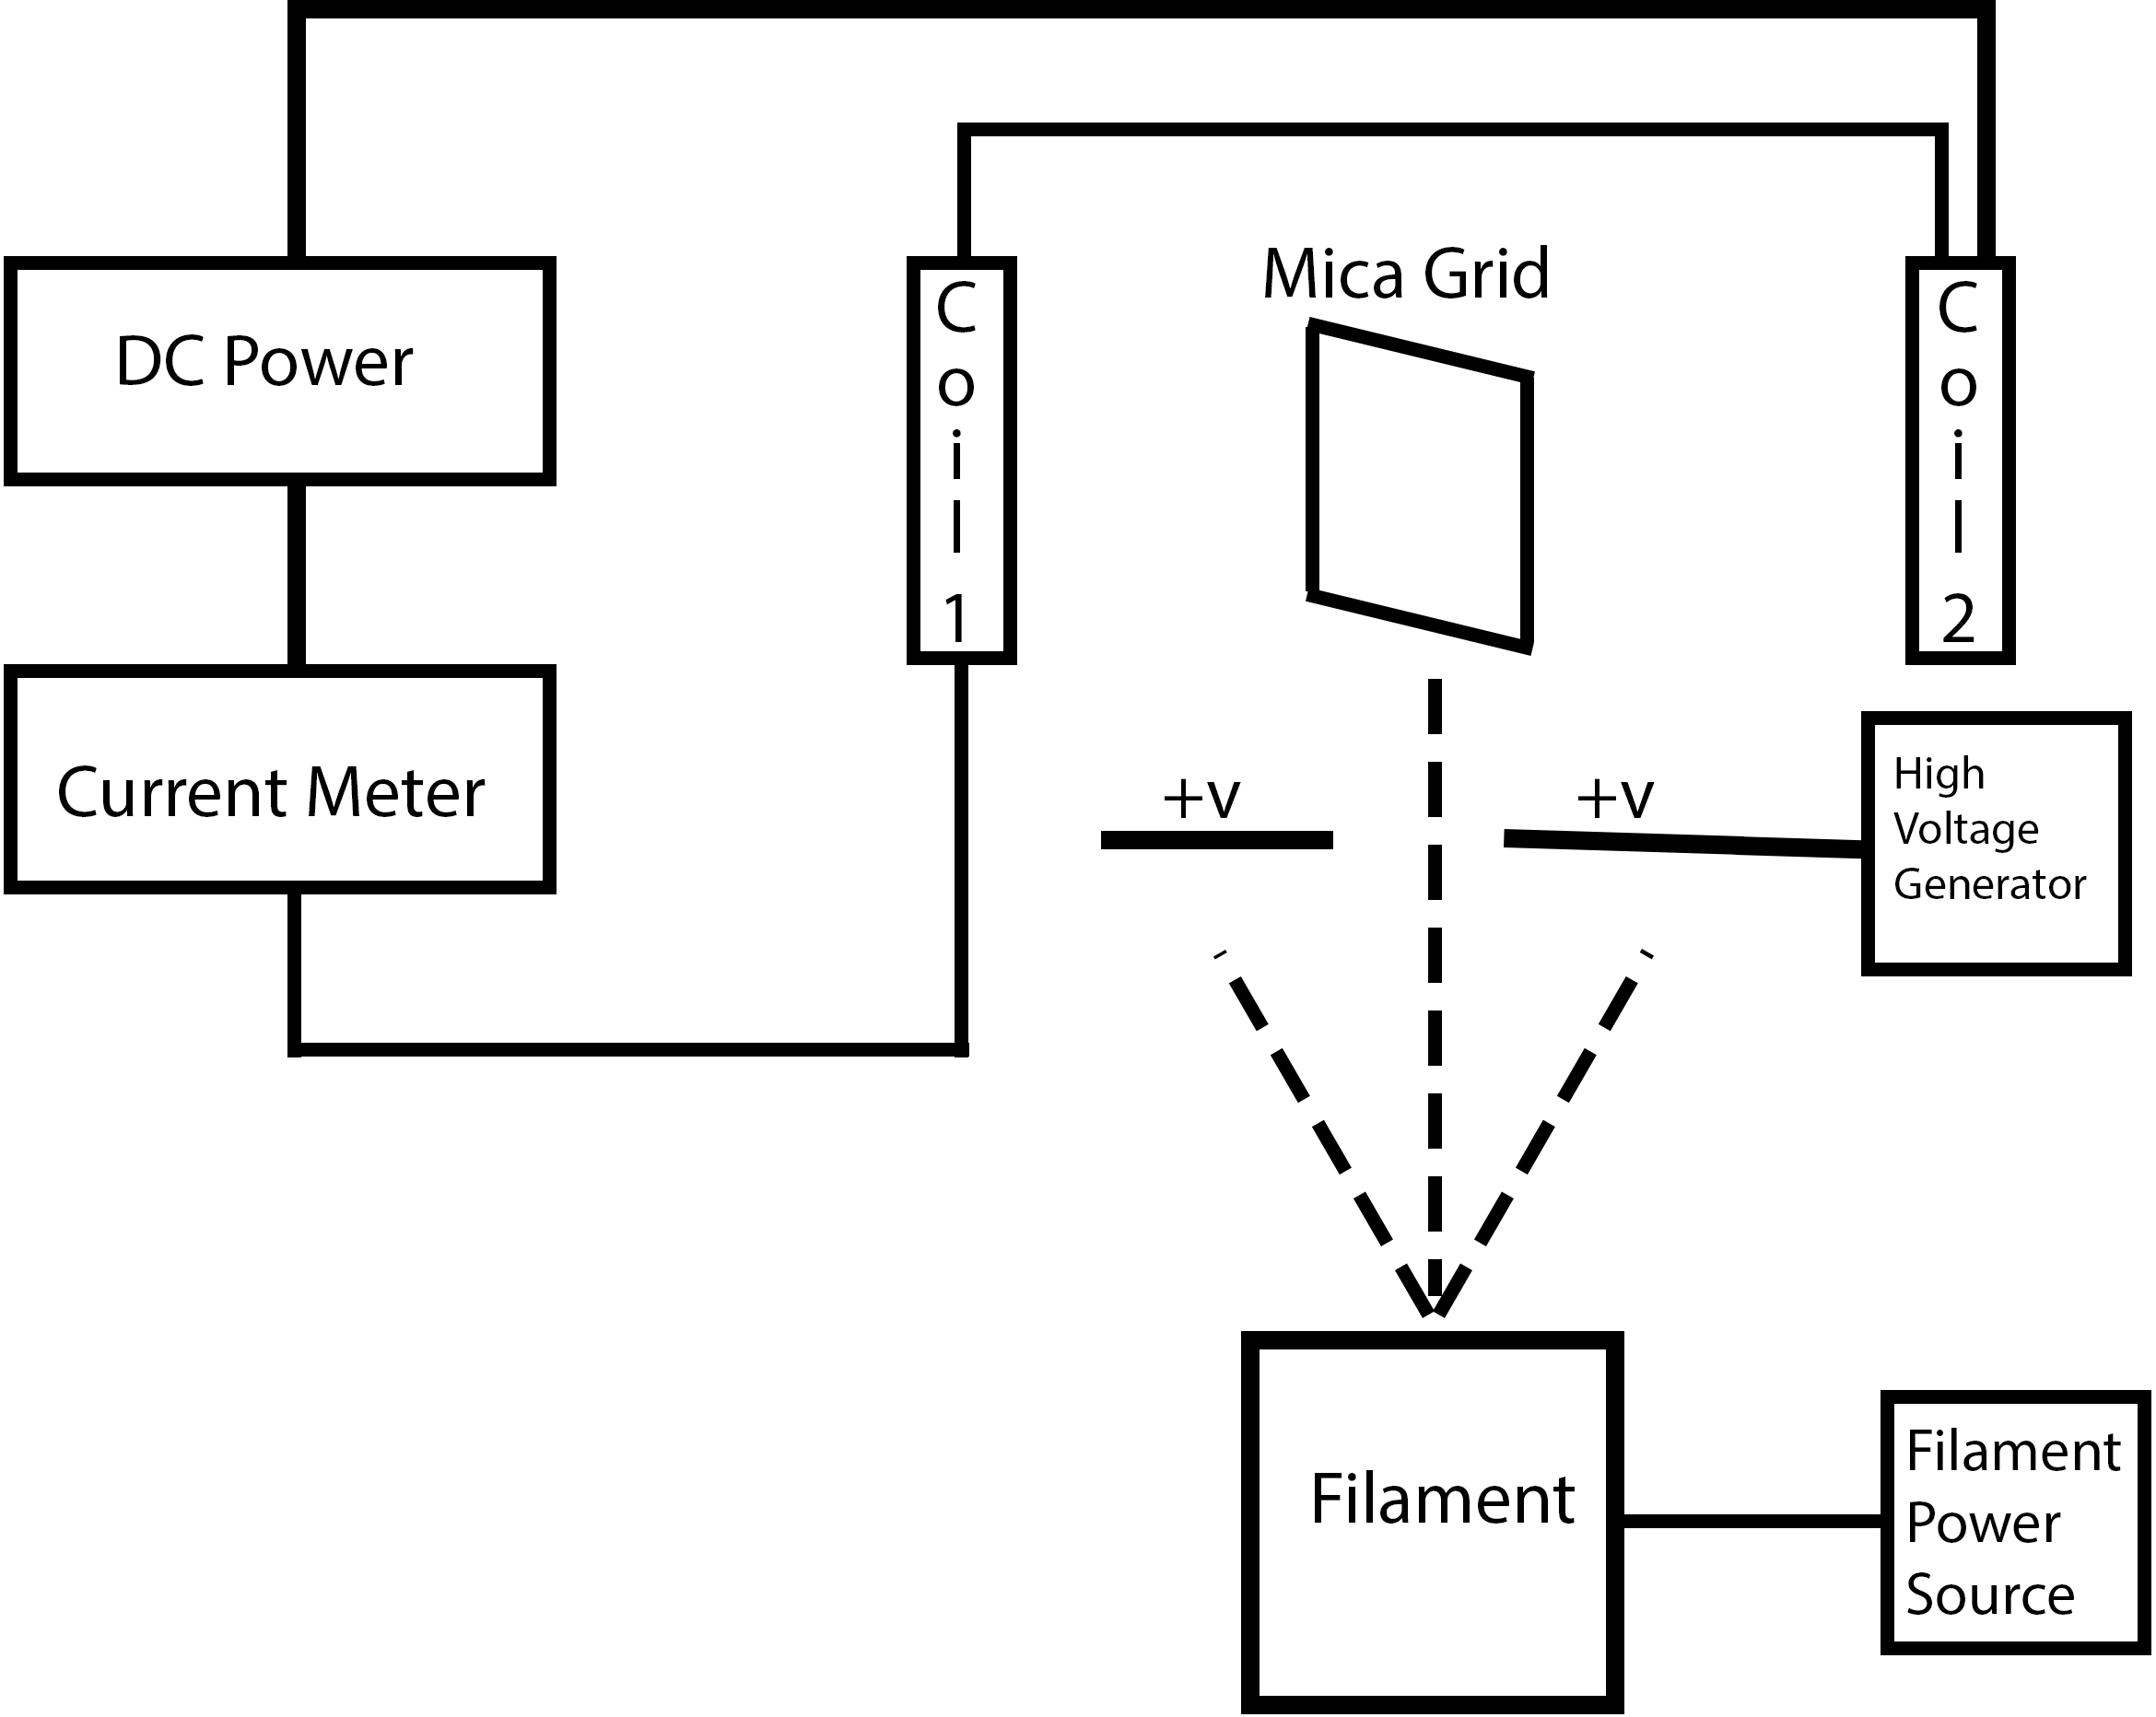
\includegraphics[width=.6\textwidth]{BlockDiagram.png}
  \caption{Schematic of the experimental setup. The Mica grid was also partially enclosed by two electrodes at $+V$ to minimize the electric field in the region.}

\end{figure}

To measure the charge to mass ratio, we directed our electron beam perpendicular to the field produced by a Helmholtz coil with $N = 125$ turns and a diameter $D = 21.3 \pm .1$ cm. A DC power supply is used in series with a current meter to produce a constant and nearly homogeneous magnetic field. From the Bio-Savart law, we calculate the magnetic field produced by a Helmholtz coil:
\begin{equation}
B = \frac{16 {\mu}_o N I}{\sqrt{125}D} 
\label{BField}
\end{equation}
The electron beam is created by boiling electrons off a filament and accelerating them towards a slit that is cut into a high voltage electrode. Some electrons pass through the slit into a vacuum tube where their path is illuminated by a mica screen centered between the Helmholtz pair. The mica screen provides phosphorescent grid paper that we use to record the beam position and later determine the radius of curvature. 



	As seen in table \ref{table:1} we recorded a total of five measurements for the beam deflection in the presence of five incremental field strengths. Before taking any measurements, we noted that with zero applied field our beam was slightly offset by 0.05cm. To account for this, first we subtracted the offset value from our data. Additionally, we used a current reversing switch to average the measurements after switching the magnetic field sign. As is necessary to determine the magnetic field due to a pair of Helmholtz coils, we also measured the current through the coils for each data set.
    
\begin{table}[h!]
\centering
\caption{Vertical Beam Deflection}
\label{my-label}
\resizebox{\textwidth}{!}{%
\begin{tabular}{|l|l|l|l|l|l|}
\hline
 & \begin{tabular}[c]{@{}l@{}}$V_a$ = 1000 $\pm$ 1 V \\ I = .31 $\pm$ .01 A\end{tabular} & \begin{tabular}[c]{@{}l@{}}$V_a$ = 1500 $\pm$ 1V \\ I = .38 $\pm$ .01 A\end{tabular} & \begin{tabular}[c]{@{}l@{}}$V_a$ = 2000 $\pm$ 1V \\ I = .44 $\pm$ .01 A\end{tabular} & \begin{tabular}[c]{@{}l@{}}$V_a$ = 2500 $\pm$ 1 V \\ I = .49 $\pm$ .01 A\end{tabular} & \begin{tabular}[c]{@{}l@{}}$V_a$ = 3000 $\pm$ 1V \\ I = .54 $\pm$ .01 A\end{tabular} \\ \hline
x (cm) & y $\pm$ .05 cm & y $\pm$ .05 cm & y $\pm$ .05 cm & y $\pm$ .05 cm & y $\pm$ .05 cm \\ \hline
2 & .163 & .125 & .150 & .150 & .175 \\ \hline
4 & .438 & .425 & .425 & .450 & .450 \\ \hline
6 & .850 & .825 & .825 & .850 & .850 \\ \hline
8 & 1.375 & 1.350 & .135 & 1.375 & 1.350 \\ \hline
10 & 2.050 & 2.025 & 2.025 & 2.025 & 2.050 \\ \hline
\end{tabular}%
}
\label{table:1}
\end{table}

We observed the ray trajectory to be nearly the same for each data set despite variations in both current and accelerating voltage. This coincidence is resolved upon further inspection of equation \ref{Energy}. The radius of curvature depends  on the ratio $\frac{\sqrt{V_a}}{I}$, which is a consistent value of approximately 100 for all our measurements.
    
\section{Procedures and Data}
We proceed to analyze the measured values for points in the electron path by performing a least squares fit to the general equation of a circle. 

\begin{figure}[h!]
  \centering
  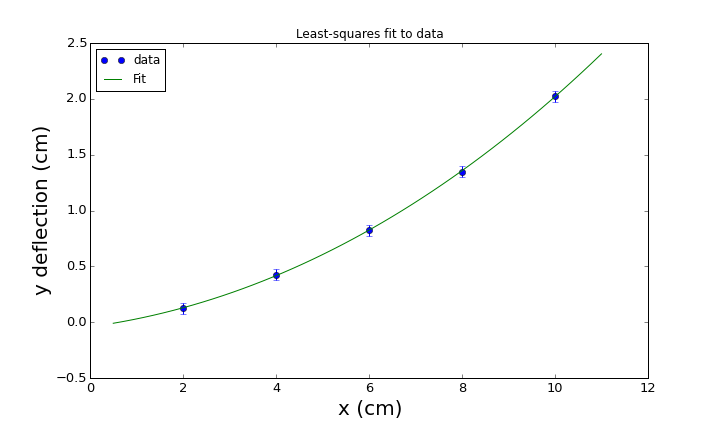
\includegraphics[width=1\textwidth]{Sample.png}
  \caption{Curve fitting results for the 1000V data set as seen in table \ref{table:1}. }
\label{Curve}
\end{figure}

The optimization algorithm returns the radius of curvature for each data set shown in table \ref{table:1}. Once the radius is calculated, we can rearrange the combination of equation \ref{BField} and equation \ref{Energy} to determine the charge to mass ratio: 

\begin{equation}
\frac{e}{m} = \frac{125}{128}\frac{V_a D^2}{{{\mu}_o}^2 N^2 I^2 r^2} 
\end{equation}

As seen in figure \ref{Curve}, our raw data is in good agreement with the accepted value of $1.77x10^11 C/kg$. Uncertainties were calculated using the standard methods of error propagation as outlined in Taylor's Error Analysis text \cite{Taylor1997AnAnalysis}. There were three main sources of uncertainty that we considered. The fitting algorithm contributed $7\% $ fractional uncertainty for the path radius and the diameter of our Helmholtz coils could not be determined with precision greater than 0.1cm. Ideally the current source would supply a negligible amount of uncertainty, but early inspection of the apparatus revealed current fluctuations, presumably due to a frayed cable. Although fluctuations vanished when the cable was replaced, we choose to be cautious and prescribe an uncertainty of 0.1 Amps to all current measurements. 

\begin{figure}[h!]
  \centering
  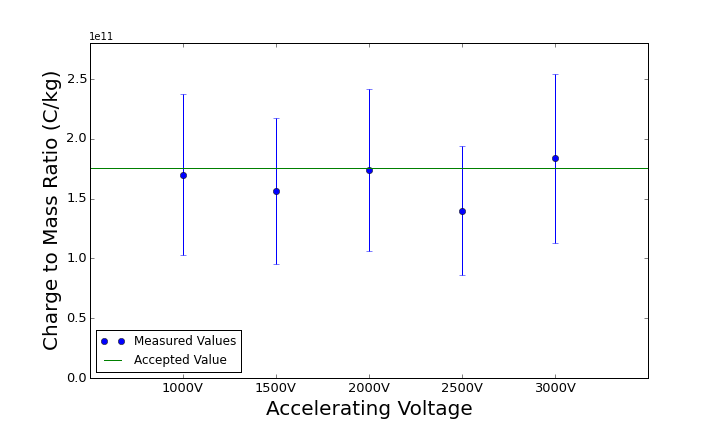
\includegraphics[width=1\textwidth]{Results.png}
  \caption{Plot of the resulting measurements when compared to the accepted value.}
\label{Results}
\end{figure}

An average of the five data points shown in Figure \ref{Results}, with the standard deviation of the mean as the uncertainty, provides the final result of $(1.648 \pm .287)$x$10^{11} C/kg$ for the charge to mass ratio of the electron. This result is greatly significant because it demonstrates that cathode rays are simply negatively charged massive particles. It is not necessary fall back on aether theory as it is more probable that the electron's circular trajectory is merely a requirement of the Lorentz Force law.



	
        
\section{Conclusion}
Our results are satisfactory, as we have verified the accepted value for the charge to mass ratio of an electron. There was little discrepancy in our calculated data and all results lie within one standard deviation of the target. Historically, the results of these measurements were interpreted and extended to the hypothesis that electrons were fundamental components of molecules. Thomson suggested that the electrons from the gas were dissociated from atoms and projected by the electric field through his tube \cite{Thomson2010CathodeRays}. Additionally, a charge to mass ratio on the order of $10^{11}$ signifies the possibility that one of these quantities may be very large or very small. Future experiments may take great interest in independently determining the charge and mass.

\bibliographystyle{plainnat}
\bibliography{Mendeley.bib}



\end{document}